\subsection{Problem Statement}

The best way to understand how neural networks work is to build one yourself from scratch. The understanding becomes even more comprehensive if there is a particular problem that can be solved using NNs. Therefore let's start our work by taking a look at Figure \ref{fig:digit-classification}.

\begin{figure}[H]
    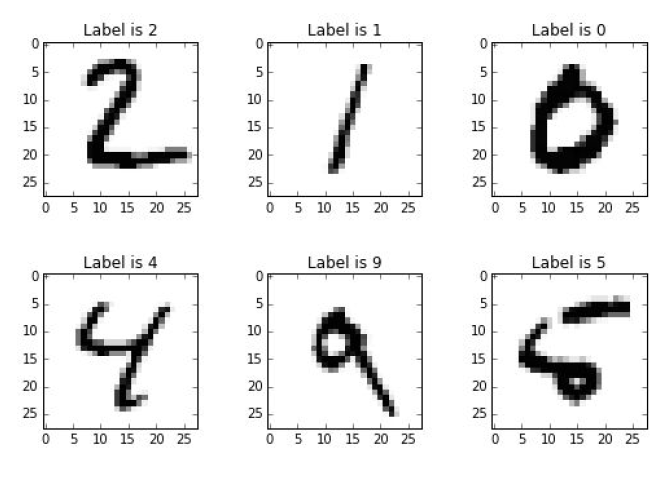
\includegraphics[width=\linewidth]{pics/problem.png}
    \caption{\label{fig:digit-classification} Digit Classification Problem}
\end{figure}

There are handwritten numbers that you want computer to correctly classify. This would be an easy task for a person but at least for a long period of time was an extremely complicated one for a machine. 

Even though the computer is faster than the human brain in numeric computations, the brain outperforms the computer in some other tasks. Many of those tasks are related to the human ability for sentience (which is a concept different from intelligence). The trick is to find a way, so that the computer could apply its numeric computation skills to solve these later tasks (at least to some degree).

The first step would be to limit the scope of the task. In our particular case the broad task of image recognition will be addressed as a classification problem - a task of giving an object a label from a given set of labels.

As we will see during the process of building our own NN, its output is based almost exclusively on application of linear algebra methods. Despite the name (which is sometimes related to the fear of artificial intelligence), neural networks in fact are much more related to statistical methods (like regression analysis or curve fitting) than to the way human brain works (\cite{reid2014}). 

NNs are inspired by human brain only to certain extent. For instance the main element that makes them similar is a multilayer net structure of simple elements that are connected in some way, receiving and transmitting information. But the structure of the human brain is much more complicated, besides it is self-organizing and adaptive in contrast to the fixed manually designed architecture of a NN. Hence, there is a good reason to stop being afraid of neural networks and instead to create one ourselves.

\begin{figure}[H]
    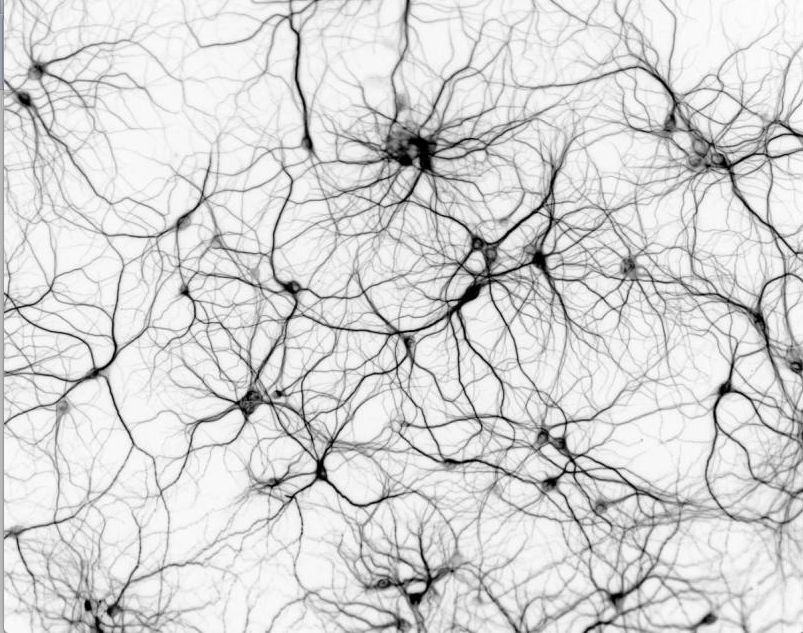
\includegraphics[width=\linewidth]{pics/neurons_net3.png}
    \caption{\label{fig:real-neurons} Brain Neurons. Source: pixabay.com}
\end{figure}


\subsection{Schematic Representation}
A complex multilayer structure that all neural networks have in common in a simplified way can be depicted using the Figure \ref{fig:nn-schema}.

\begin{figure}[H]
    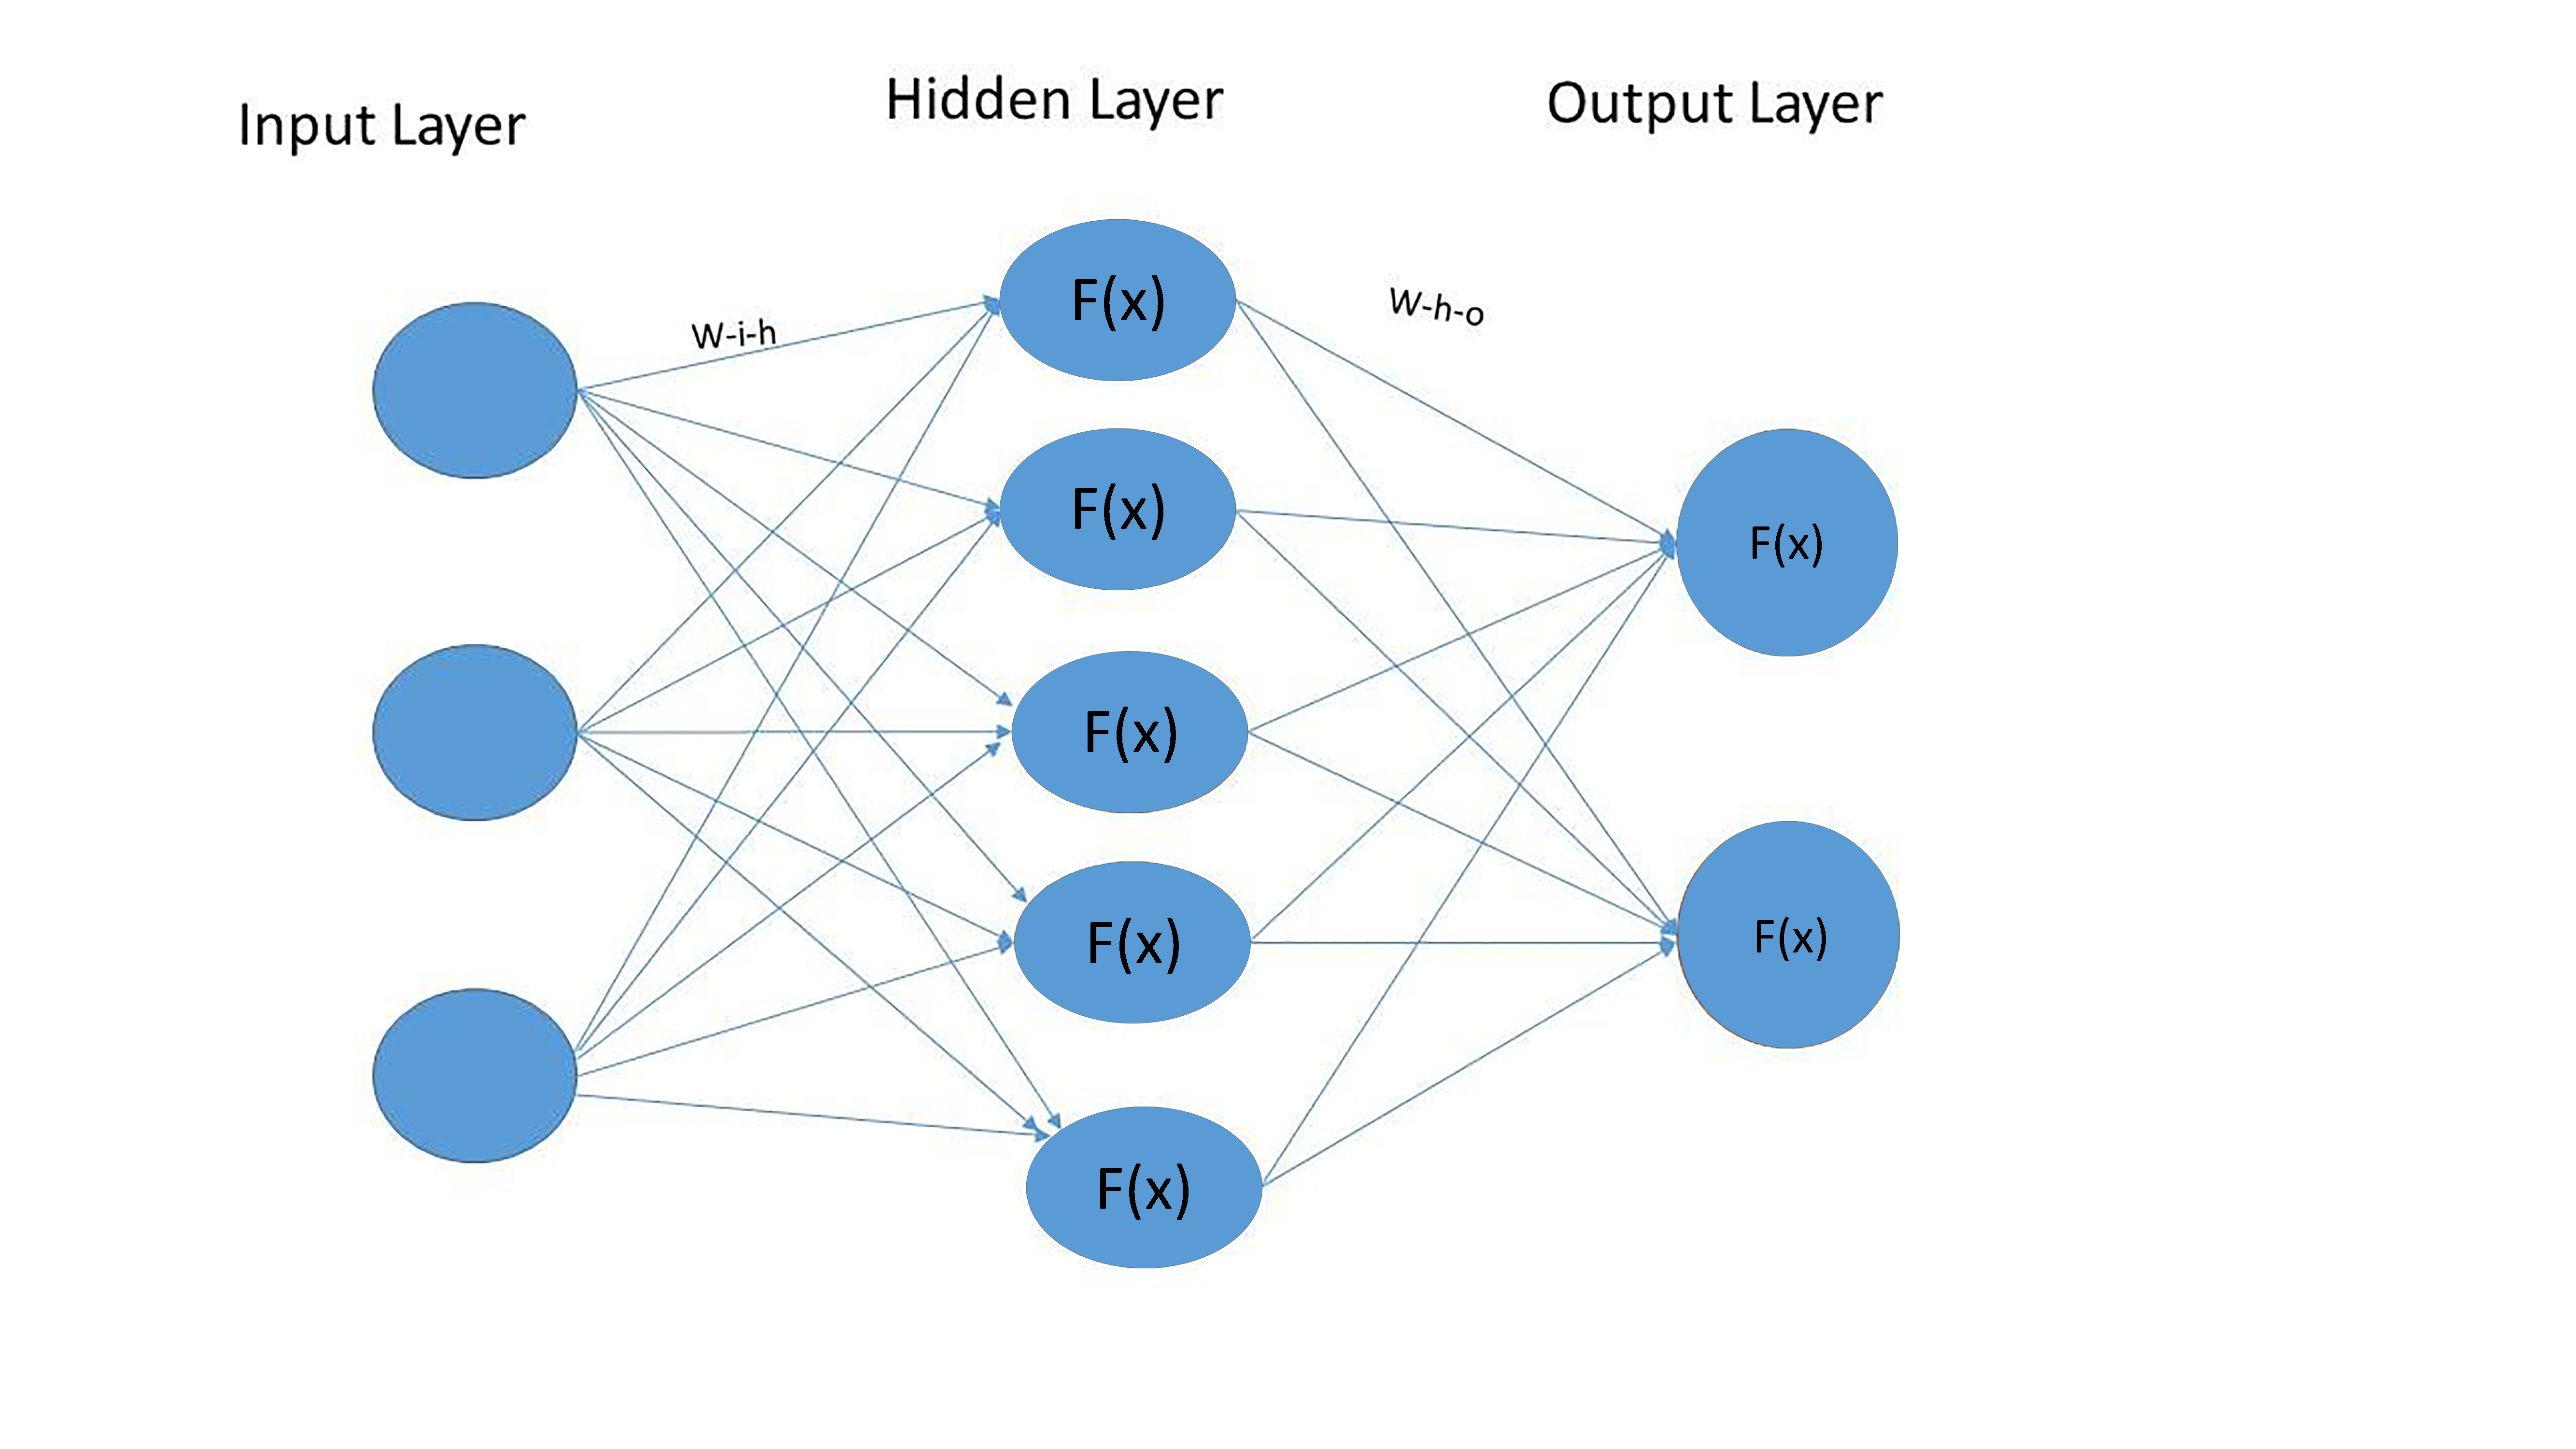
\includegraphics[width=\linewidth]{pics/neural_network1.jpg}
    \caption{\label{fig:nn-schema} Neural Network Schema}
\end{figure}

All we need in order to implement such a structure is base Python and numpy, a library for numerical computation, which we will be using to do linear algebra. 

First let's determine the elements of a neural network depicted on the Figure \ref{fig:nn-schema}: nodes, layers, weights across nodes and activation functions.

\begin{itemize}
    \item \textbf{Nodes}. A node is basically a point where data points are received, processed and then transferred to the node. A node could be either an endpoint or a redistribution point or even both when iterations are done through the learning algorithm. The number of nodes to use is optional.

    \item \textbf{Layers}. A layer consists of one or several nodes. The initial layer in the network is called the input layer and it is the entry point through which the data is fed into the neural net. The middle layers are called hidden layer because the computation results of them are not directly visible to someone interacting with the neural net. In the hidden layers, which can range from one to thousands, the features are transformed and most of the structure (both linear and nonlinear) is captured. Finally, there is the final layer, from which results are output. The nodes in each layer are fully interconnected to the ones in the next and the previous layers. 


In our case we have a structure with 3 layers: input, output and one hidden layer. The number of nodes in the input  (i\_n), hidden (h\_n) and output (o\_n) layers are 3, 5 and 2 respectively. In Python, such a structure can be represented in the following way:

\begin{lstlisting}[language=Python]
    # Load the package to work with numbers
    import numpy as np
    
    # Determine the structure of the NN
    i_n = 3
    h_n = 5
    o_n = 2
\end{lstlisting}

    \item \textbf{Weights.} In order to transfer an input data point to the next layer, a predetermined number (called weight) is stored in each connection from the sender node to the receiver node. Each weight accounts for the impact between the interconnected nodes. Initially, we assign weights between nodes in neighboring layers randomly. This is needed only for the sake of initializing the structure. Later these weights will be changed in order to solve our classification problem. The weight updating will be better described in the following sections. Neural nets will have n-1 matrices of weights, where n is the number of layers in the NN. You can imagine these weight matrices sitting between two layers representing the strength of the connection between every single node of neighboring layers. Thus, each of these matrices will be of size f x p, where p is the number of nodes in the preceding layer and f is the number of nodes in the following layer.
    This becomes more clear once you check the code below that creates 2 matrices of weights: the 5x5 matrix of weights between input and hidden layers (w\_i\_h) and the 2x5 matrix of weights between hidden and output layers (w\_h\_o). Such a dimensions of matrices are necessary in order to accomplish matrix and vector multiplications that are done in the following stages.

\begin{lstlisting}[language=Python]
    # Randomly define the weights between the layers. 
    w_i_h = np.random.rand(h_n, i_n) # create an array of the given shape and populate it with random values.
    w_h_o = np.random.rand(o_n, h_n) 
    
    # Show matrices of randomly assigned weights.
    w_i_h
    # w_h_o # uncomment this line in order to see the values for w_h_o.
    # Use Cmd + / in MacOS and CTRL + / in MS Windows as a shortcut to comment/uncomment lines.
\end{lstlisting}

\begin{lstlisting}
    array([[0.63964736, 0.97236245, 0.83944375],
    [0.31439566, 0.54254369, 0.0456713 ],
    [0.93759599, 0.71292359, 0.11961199],
    [0.90587079, 0.0855728 , 0.55046849],
    [0.89559465, 0.47349711, 0.42168825]])
\end{lstlisting}

\item \textbf{Activation Function.} The remaining element of the NN's structure is an activation function - a function which transforms an input data point that it receives from the previous nodes to an output value which will be the input for the nodes in the next layer. The activation function plays an important role in the efficiency of the neural network as it accounts for non-linearity of data. 
It is to certain extent inspired by the concept of firing, which means that neurons fire or transmit information further only if the input surpasses certain threshold. The simplest activation function can be represented by a step function as on the Figure \ref{fig:act-fct}. 

\begin{figure}[H]
    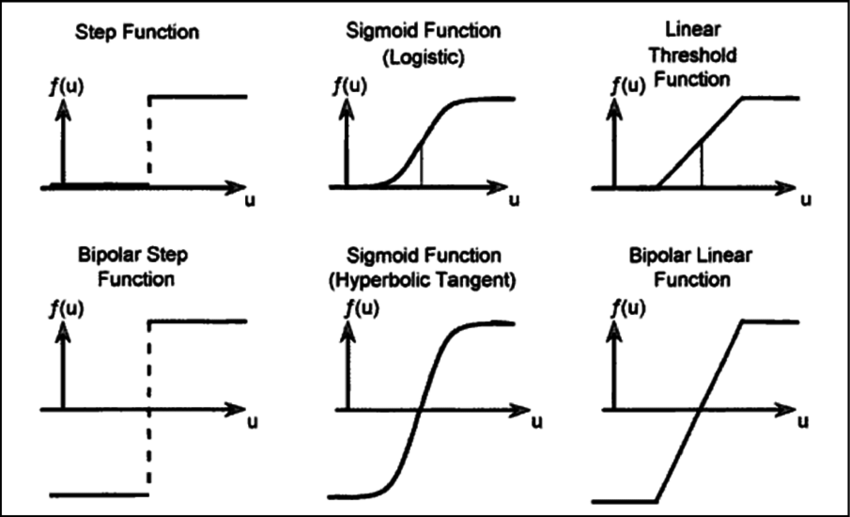
\includegraphics[width=\linewidth]{pics/step_function.png}
    \caption{\label{fig:act-fct} Activation Functions. Source: Research Gate}
\end{figure}

In our NN, we will use a slightly more elaborate activation function, the sigmoid function (logistic), which allows for more efficient use of the input data. A description of various activation functions, their benefits and disadvantages is given in sections below.

\begin{lstlisting}[language=Python]
    # Determine activation function.
    def sigmoid(x):
        # np.exp() calculates the exponential
        # of all elements in the input array.
        return 1 / (1 + np.exp(-x)) 

    # Draw activation function.
    import matplotlib.pyplot as plt
    
    # return 100 evenly spaced numbers over an interval from -10 to 10.
    x = np.linspace(-10, 10, 100) 
    # plot sigmoid function for sampled values.
    plt.plot(x, sigmoid(x)) 
    plt.show()
\end{lstlisting}

\begin{figure}[H]
    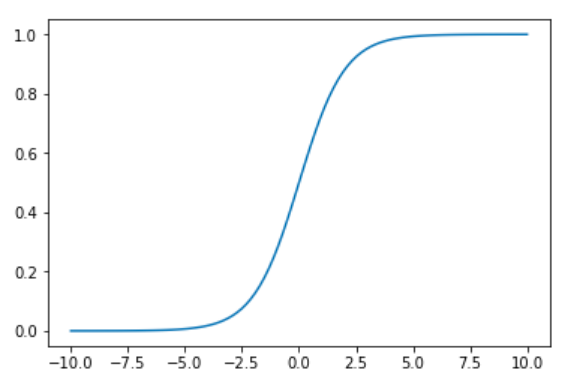
\includegraphics[width=\linewidth]{pics/sigmoid.png}
    \caption{\label{fig:sigmoid-fct} Sigmoid Function}
\end{figure}

\end{itemize}


\subsection{Data Inspection}

By now we have collected all the elements of the NN. Can we use this structure in order to solve the classification problem stated in the beginning? In order to answer this question we need first to get a better understanding of the data at our disposal. 

We are trying to check whether NN is able to solve the classification problem using a collection of 70 000 handwritten numbers. Each of this handwritten number is represented as 28x28 image. 

The original source of the data is THE MNIST DATABASE. In the links below, you can find: 

\begin{itemize}
    \item http://yann.lecun.com/exdb/mnist/: A detailed description of the dataset and a summary of the performance results achieved by various classification algorithms.
    \item https://pjreddie.com/projects/mnist-in-csv/: the data we will use. Here the original images are saved in CSV, which allows to work with them directly.
\end{itemize}

For the purposes of demonstration below we use a smaller dataset (100 images), which will be expanded at a later stage.


\begin{lstlisting}[language=Python]
    # Load the data.
    # "r" stands for "read only" mode.
    raw_data = open("data/mnist_train_100.csv", 'r') 
    # read all the lines of a file in a list.
    data = raw_data.readlines() 
    # remove temporal file from the environment in order to save memory.
    raw_data.close() 

    # Inspect the data - check the number of observations.
    # length of the object.
    len(data) 
\end{lstlisting}

\begin{lstlisting}
    100
\end{lstlisting}

\begin{lstlisting}[language=Python]
    # Inspect a particular observation of the data.
    # show observation number 0 from the list
    # (remember that in Python numbering starts from 0).
    data[0]
\end{lstlisting}

\begin{lstlisting}[language=Python]
'3,0,0,0,0,0,0,0,0,0,0,0,0,0,0,0,0,0,0,0,0,0,0,0,0,0,0,0,0,0,0,0,0,0,0,
0,0,0,0,0,0,0,0,0,0,0,0,0,0,0,0,0,0,0,0,0,0,0,10,254,254,254,254,255,209,
126,67,32,0,0,0,0,0,0,0,0,0,0,0,
...
254,233,139,57,232,254,243,166,28,0,0,0,0,0,0,0,0,0,0,0,0,0,0,0,0,0,0,0,0,
0,0,0,0,0,0,0,0,0,0,0,0,0,0,0,0,'
\end{lstlisting}

From the result above, we see that 1) a particular observation looks like a string of 785 elements (label of the image + 784 elements for each pixels of a 28x28 image), 2) each element representing a pixel is a number from 0 to 255 (from white to black color) and 3) the first element in the line is the label of the image and therefore is a number from 0 to 9.

Using `matplotlib`, we can also reconstruct the original image based on the data about each pixel in the string.

\begin{lstlisting}[language=Python]
    # Load the package to plot the data
    import matplotlib.pyplot as mpp

    # Plot the data
    observation = data[0].split(',') # break down observation number 0 (comma is used to identify each element).
    image = np.asfarray(observation[1:]).reshape((28,28)) # take all the elements starting from the element 1 
    # (exclude element number 0, that corresponds to the label) and reshape them as an array with dimension 28 by 28.
    mpp.imshow(image, cmap='Blues', interpolation='None') # show the plot of this array using grey pallete.

    # Save an observation of the data as an input to work with.
    input = np.array(np.asfarray(observation[1:]), ndmin=2).T # save necessary elements in a vertical vector shape.
\end{lstlisting}

\begin{figure}[H]
   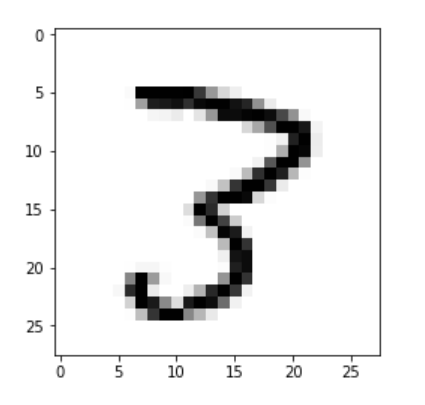
\includegraphics[width=\linewidth]{pics/3.png}
   \caption{\label{fig:number3} Plot of the handwritten number}
\end{figure}

    \subsection{Fitting the Structure of the NN to the Data}

After inspecting the data, we can conclude that the structure in Figure \ref{fig:nn-schema} with 3-5-2 nodes is probably not optimal and therefore should be updated in order to fit the data we have and peculiarities of the classification problem: 

\begin{itemize}
    \item For each observation we have 784 elements as an input (label element is excluded). Accordingly, instead of 3 input nodes we should better have 784.
    \item Similarly, as we have 10 different options for the outcome (handwritten numbers are labeled from from 0 to 9) the number of output nodes should be 10 instead of 2. 
    \item We also change the number of hidden nodes from 5 to 90. Such a number has been assigned based on some proportionality assumptions which will be checked later: 90 is 9 times higher than 10 and approximately 9 times smaller than 784.
\end{itemize}

As we have new structure of the NN we should reassign the weights - now the size of each weight matrix will increase as we have more nodes in each layer.

\begin{lstlisting}[language=Python]
    # Determine the new structure of the NN.
    i_n = 784
    h_n = 90
    o_n = 10
    
    # Determine the weights.
    w_i_h = np.random.rand(h_n, i_n)
    w_h_o = np.random.rand(o_n, h_n)
\end{lstlisting}

So far we have not used the first element of our observation - the label. It will be necessary to compare the predictions of the NN to the real state of the world and to train the NN to make correct predictions. The target should therefore have the same shape as the output layer of the NN, so that they could be comparable. We can represent the label as a vector of n binary (0 or 1) elements (n corresponds to the number of nodes in the output layer). There should be only one element equal to 1 and the position of this element should correspond to the index number of the label we want to predict.

\begin{lstlisting}[language=Python]
    # Create target array.
    target = np.array(np.zeros(o_n), ndmin=2).T
    # int() method returns an integer object
    # from any number or string.
    target[int(observation[0])] = 1 

    # Inspect how the target looks like (remember that the label of observations is 5).
    target

    # Show the sizes of matrices of weights, input and target vectors.
    w_i_h.shape, input.shape, w_h_o.shape, target.shape
\end{lstlisting}

\begin{lstlisting}
((90, 784), (784, 1), (10, 90), (10, 1))
\end{lstlisting}

\subsection{Feedforwarding}

Once we have the structure of the NN updated for the specific task of classifying the numbers depicted on the images, we can run our network in order to get the first predictions that will be represented by a vector of 10 elements. This vector in its turn can be compared to the target.

To run the NN, i.e. to feed forward our input data in order to get some predictions, we should follow certain steps:

\begin{enumerate}
    \item Multiply an input vector by a matrix of weights that connects it with the next layer;
    \item Transform the result using activation function;
    \item Use the output obtained in the 2nd step as an input vector for the next layer.
\end{enumerate}

A sequence of this steps should be repeated n-1 times (where n corresponds to the number of layers). The output of the previous layer will always be the input vector for the next layer. In our case the procedure will happen twice.

In the Figures \ref{fig:multiplication} and \ref{fig:activation}, you can see the procedure necessary to obtain the output of the hidden layer. The result of matrix multiplication here is called Hidden\_Input. Result of the transformation of Hidden\_Input through activation function is called Hidden\_Output.

This output will be used as the input vector that should be multiplied by the next weight matrix and transformed through activation function in order to calculate the final output of the NN. If our NN would have more than one hidden layer, the procedure would be repeated more times.

\begin{figure}[H]
    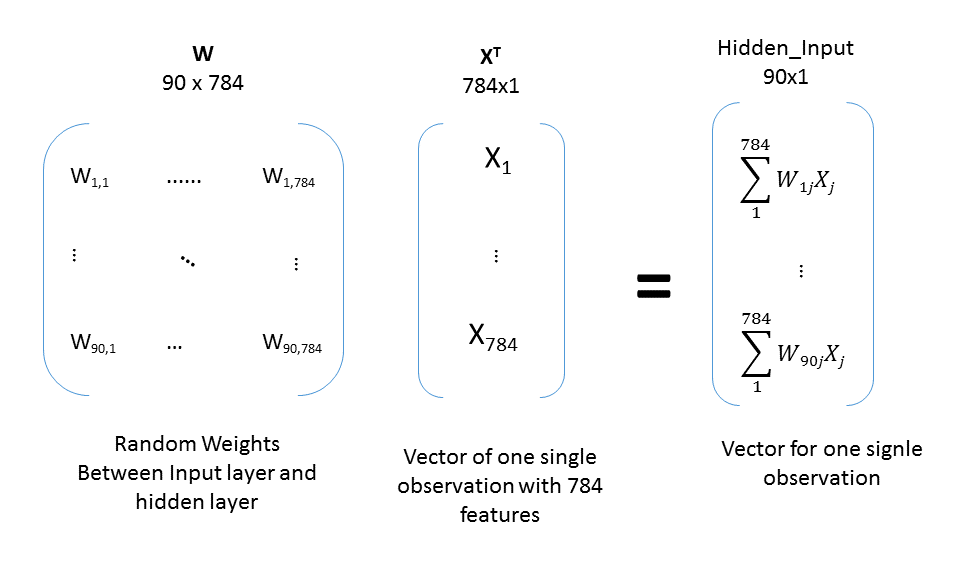
\includegraphics[width=\linewidth]{pics/multiplication.png}
    \caption{\label{fig:multiplication} How Weights Work}
\end{figure}

\begin{figure}[H]
    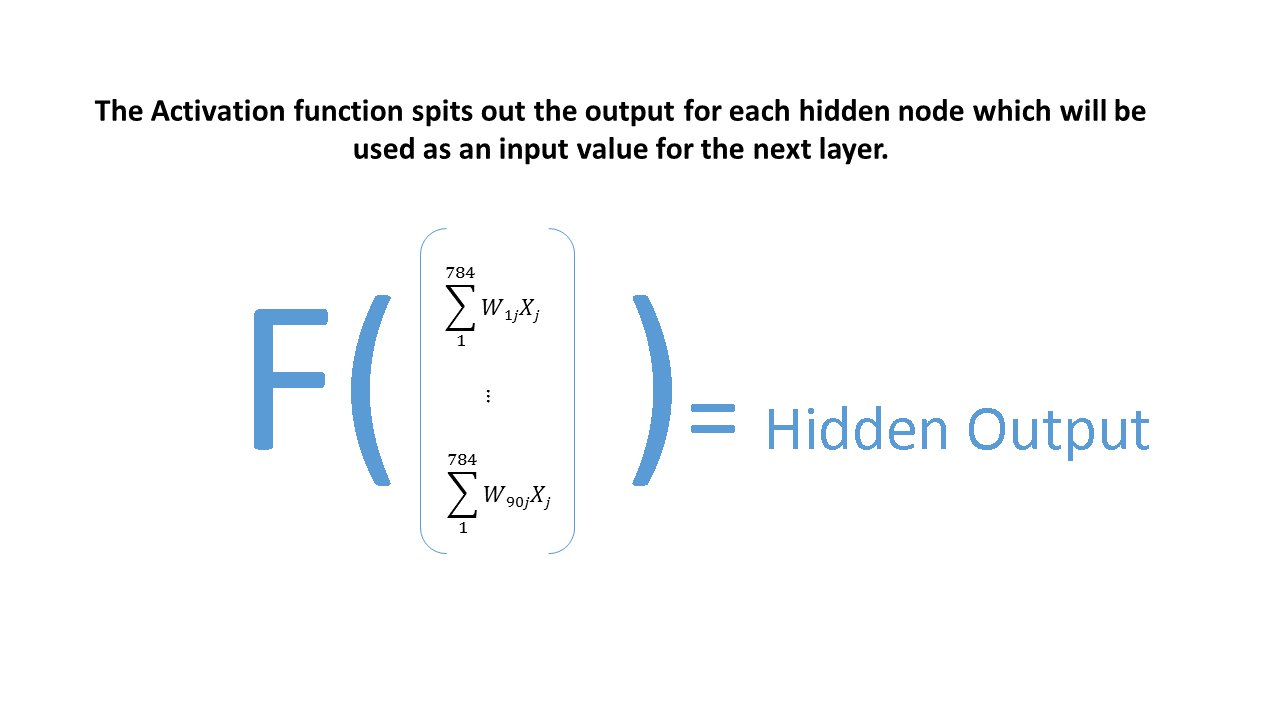
\includegraphics[width=\linewidth]{pics/activation.jpg}
    \caption{\label{fig:activation} How Activation Works}
\end{figure}

Below you can see the code implementation of all the steps for all layers of the NN.

\begin{lstlisting}[language=Python]
    # Calculate the output of hidden and output layers of our NN.
    # dot() performs matrix multiplication; "h_input" stands for "Hidden_Input".
    h_input = np.dot(w_i_h, input) 
    # "Hidden_Output" - result after activation function.
    h_output = sigmoid(h_input) 
    # "Output_Input" - input used for the next layer.
    o_input = np.dot(w_h_o, h_output)
    # "Output_Output" - final output of the NN.
    o_output = sigmoid(o_input)

    # Print output to the screen
    o_output 
\end{lstlisting}

\begin{lstlisting}
    array([[ 1.],
    [ 1.],
    [ 1.],
    [ 1.],
    [ 1.],
    [ 1.],
    [ 1.],
    [ 1.],
    [ 1.],
    [ 1.]])
\end{lstlisting}

\subsection{Good Practices on Data Treatment}

Once we check the output of the NN and the results of each performed step, we can observe that already at the stage of the h\_output all the data converts to a vector in which all the values are equal to 1. Such a vector does not provide us with any helpful insight. Apparently, something is wrong with what we have done so far. There could be several reasons for the problem we face. Take a look at our sigmoid function in Figure \ref{fig:sigmoid-fct}.

\begin{figure}[H]
    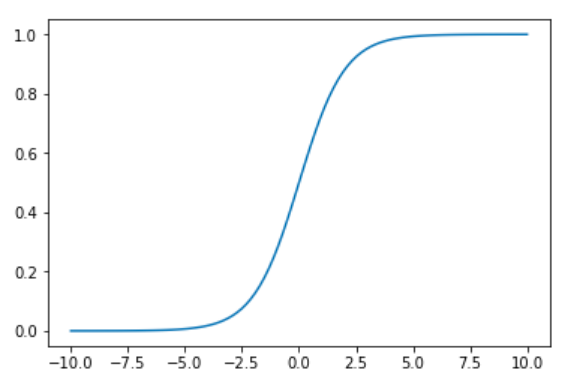
\includegraphics[width=\linewidth]{pics/sigmoid.png}
    \caption{\label{fig:sigmoid-fct} Sigmoid Function}
\end{figure}

As we can see the output of the sigmoid function will be almost identical once we feed a number bigger than 2. Similarly there is no significant difference between the outputs if numbers used are smaller than -2. Hence the application of sigmoid function to the original data leads to a loss of valuable information. The NN has problems learning something from the inputs, which are almost undifferentiable.  

One solution is to transform the input we have. Ideally we should have our data in a range between 0 and 1. It is also desirable to avoid zeros as inputs, because the output of a zero input will always be zero, no matter how large the weights are, in which case the NN will not be able to use this input to learn.

We can perform a transformation of the original data as the one coded below.

\begin{lstlisting}[language=Python]
    # Good practice transformation of the input values:
    input = np.array((np.asfarray(observation[1:])/255.0*0.99) + 0.01, ndmin=2).T 
    # Our values in our input vector are in the range from 0 to 255. Therefore we should divide input vector by 255, 
    # multiply it by 0,99 and add 0,01 in order to get values in the range from 0,01 to 1.
    
    # Good practice transformation of the target value:
    target = np.array(np.zeros(o_n) + 0.01, ndmin=2).T
    target[int(observation[0])] = 0.99
\end{lstlisting}

Secondly, we can check our way to randomly assigned initial weights. Let's take a look once at the function we used to randomly assign them.

\begin{lstlisting}[language=Python]
    np.random.rand(3, 5)
\end{lstlisting}

\begin{lstlisting}
    array([[ 0.22583725,  0.12109248,  0.02590624,  0.12690234,  0.62018663],
    [ 0.81179976,  0.46311266,  0.71892529,  0.44099911,  0.43754171],
    [ 0.49648974,  0.30002541,  0.04783774,  0.69393036,  0.58613769]])
\end{lstlisting}

As we can see, all the weights are positive, while the actual relationship between the features in the data and the values of the output vector can be negative. Hence, the way we employ to assign random weights should allow for negative weights too.

Below there are too alternatives how this can be implemented in Python.

\begin{lstlisting}[language=Python]
    # Good practice for initial weights assignment:
    
    alternative1 = np.random.rand(3, 5) - 0.5 
    # or
    alternative2 = np.random.normal(0.0, pow(3, -0.5), (3, 5)) 
    # arguments: Mean of the distribution, Standard deviation of the distribution, Output shape.
    # Second approach is better as it takes in account the standard deviation 
    # that is related to the number of incoming links into a node, 1/√(number of incoming links).
    
    # alternative1
    alternative2

    # Define the weights in accordance with the best practice:
    w_i_h = np.random.normal(0.0, pow(h_n, -0.5), (h_n, i_n))
    w_h_o = np.random.normal(0.0, pow(o_n, -0.5), (o_n, h_n))
\end{lstlisting}

Now that we have all the elements assigned in accordance with good practices, we can feedforward the data once again and evaluate the results by comparing the predictions to labels.

\begin{lstlisting}[language=Python]
    # Run NN to get new classification of the particular observation:
    h_input = np.dot(w_i_h, input)
    h_output = sigmoid(h_input)
    o_input = np.dot(w_h_o, h_output)
    o_output = sigmoid(o_input)

    # Calculate the errors of the classification:
    o_errors = target - o_output
    o_errors
\end{lstlisting}

\begin{lstlisting}
    array([[-0.06373055],
    [-0.13887152],
    [-0.95694188],
    [ 0.28799234],
    [-0.23295729],
    [-0.21478192],
    [-0.74462671],
    [-0.65361842],
    [-0.36623992],
    [-0.46408493]])
\end{lstlisting}

The result we would like to achieve should look like a vector of values where almost all values are negligibly small except for the one value that has the position in the vector corresponding to the index of the true label. 

It is not the case now. Nevertheless, one should remember that so far all the weights have been assigned randomly and no training has been performed. In any case, it is not a vector of ones anymore, which an improvement.

Thus, we can proceed to the next stage, which is to find out where the errors come from and how they can be minimized.